\documentclass{article}
\usepackage{graphicx} % Required for inserting images
\usepackage{caption}
\usepackage{subcaption}
\usepackage{float}
\usepackage{amsmath}

\title{Strategies in Motion: Analyzing the Impact of Lane Changing on Traffic Dynamics}
\author{Olof Tingskull}
\date{January 2024}

\begin{document}
\maketitle

\section{Introduction}
This report explores the intricate dynamics of traffic flow and the impact of various lane-changing strategies on overall traffic efficiency. We simulate vehicular movement on a multi-lane, periodic road, where vehicles are characterized by continuous a position,  velocity. By employing the Euler Forward Method for position and velocity updates, the model tracks each vehicle's behavior in response to surrounding traffic conditions. The focus of this study is to analyze how different lane-changing strategies, namely Forward-Looking, Backward-Looking and Bi-directional, influence the flow rate and overall traffic dynamics. We incorporate elements like spontaneous braking to add realism and complexity to the simulation, enhancing our understanding of real-world traffic scenarios. The report aims to identify optimal strategies for lane changing that could potentially lead to more efficient traffic management and reduced congestion.

\section{Method}

\subsection{Model Description}
This section describes a simulation model for vehicular traffic on a multi-lane, periodic road. In this model, each vehicle is characterized by its position $p$ and velocity $v$. The vehicle dynamics are governed by discrete updates, with position and velocity evolving according to the Euler Forward Method. The position of a car at the next time step, denoted as $p_{i+1}$, is calculated using its current position $p_i$ and velocity $v_i$, and is modulated by the length of the road. This is mathematically represented as:$$p_{i+1} = (p_i + v_i \cdot dt) \bmod \textit{road length}$$ This periodicity ensures that vehicles do not leave the road, but instead re-enter at the opposite end. Similarly, a vehicle's velocity is updated considering its maximum acceleration, maximum deceleration, and a dynamically calculated \textit{target velocity}. The target velocity is a crucial safety variable, computed continuously based on the distance to the preceding vehicle. It ensures that a car can decelerate safely to avoid collision, even in scenarios where the leading car stops abruptly. The target velocity is given by:
$$\textit{target velocity} = \sqrt{2 \cdot decelaration \cdot distance}  $$
subject to the constraints:
$$ 0 \leq \textit{target velocity} \leq \textit{max velocity}$$
This model aims to prevent collisions by adjusting each car's velocity, within the bounds of zero and the pre-defined maximum velocity, according to the computed target velocity. In the event of a potential collision, the trailing vehicle will halt until its no longer colliding.

\subsubsection{Spontaneous Braking}
To introduce variability in vehicular velocities, a mechanism of spontaneous braking is incorporated. At each time step, there exists a minor probability that any given vehicle will be compelled to brake instantaneously. This aspect introduces an additional layer of complexity to the traffic dynamics, enhancing the realism of the simulation. It also underscores the strategic advantage of lane changing, particularly in response to the abrupt stopping of a preceding vehicle. The probability of spontaneous braking, refered to as Spontaneous Braking Rate, is a configurable parameter, allowing for the analysis of its impact on traffic flow.

\subsubsection{Lane chaning}
In the model, each vehicle is assigned to a specific lane and can change to adjacent lanes. Lane-changing decisions are algorithmically determined based on the following safety criteria:
\begin{itemize}
\item There must be no vehicle occupying the same road segment in the target lane, as this would result in a collision.
\item If there is an approaching vehicle in the target lane, it must be able to brake in time if the lane-changing vehicle is moving faster.
\item Post lane-change, the lane-changing vehicle must be able to brake in time if the vehicle ahead in the new lane is moving slower.
\end{itemize}
Once a vehicle determines that a lane change is feasible, it evaluates the benefits of changing lanes. The model calculates a \textit{lane score} (ranging from 0 to 1) for three options: changing to the right, to the left, or remaining in the current lane. The vehicle then selects the option with the highest score.

There are three strategies for calculating the lane score which will be assessed in this study:
\begin{itemize}
\item \textit{Forward-Looking}: The lane score is determined based on the target velocity achievable in the new lane.
\item \textit{Backward-Looking}: The lane score is determined based on the target velocity achievable by the vehicle behind the lane-changing vehicle in the new lane.
\item \textit{Bi-directional}: The lane score combines the achievable target velocities for the lane-chaning vehicle and the vehicle behind it in the new lane. This approach ensures that lane changes are beneficial for both the chaning vehicle and the trailing vehicle in the target lane.
\end{itemize}

Additionally, a bias is introduced to discourage unnecessary lane changes, favoring the vehicle's current lane. This bias significantly influences car behavior. To identify the optimal lane-chaning strategy, different bias values will be tested. The bias, refered to as Current Lane Bias, (ranging from 0 to 1), is a configurable parameter where a value of 1 signifies no lane-chaning.

\subsection{Model Configuration}
The simulation is configured a set of parameters outlined in Table \ref{table:run_config}. These parameters are integral to the behavior and outcome of the simulation, dictating the dynamics of vehicle movement and interaction within the simulated environment. Parameters are specified in standardized units, with lengths as multiples of car lengths and time measured in simulation steps.

\begin{table}[H]
\centering
\begin{tabular}{|l|p{6cm}|}
\hline
\textbf{Parameter}            & \textbf{Description} \\
\hline
Total Road Length             & \small{The length of the simulated road, expressed in multiples of a car's length.} \\
\hline
Lane Count                    & \small{The number of traffic lanes available on the road.} \\
\hline
Vehicle Density               & \small{The proportion of the road occupied by vehicles.} \\
\hline
Acceleration Rate             & \small{The rate of acceleration for vehicles. A value of 1 signifies full acceleration to maximum velocity in one time step.} \\
\hline
Deceleration Rate             & \small{The rate of deceleration for vehicles. A value of 1 signifies full deceleration to a halt in one time step.} \\
\hline
Maximum Per-Step Movement     & \small{The maximum distance a vehicle can travel in a single simulation step. This is the product of the maximum velocity and the time step (delta time).} \\
\hline
Spontaneous Stop Probability  & \small{The probability of a vehicle randomly coming to a halt at any given step.} \\
\hline
Current Lane Bias             & \small{The bias towards remaining in the current lane when evaluating potential lane-switching maneuvers.} \\
\hline
Simulation Duration (Steps)   & \small{The total number of steps (time intervals) for which the simulation will run.} \\
\hline
Lane Evaluation Strategy   & \small{The strategy used to calculate the lane score. (Bi-directional, Forward-looking, Backward-looking)} \\
\hline
\end{tabular}
\caption{Description of Simulation Parameters}
\label{table:run_config}
\end{table}

Not every possible permutation of these parameters can be practically analyzed. Therefore, the parameters are selected initially based on intuitive reasoning, observation of simulation runs, and evaluation of parameter convergence. These parameters, refered to as default parameters, are used as the basis for the remainder of this study. The default parameters are listed in Table \ref{table:default_params}.
\begin{table}[H]
\centering
\begin{tabular}{|l|p{6cm}|}
\hline
\textbf{Parameter}            & \textbf{Default Value}  \\
\hline
Total Road Length             & 200 \\
\hline
Lane Count                    & 10 \\
\hline
Vehicle Density               & 0.05 \\
\hline
Acceleration Rate             & 0.001 \\
\hline
Deceleration Rate             &  0.01 \\
\hline
Maximum Per-Step Movement     &  0.1 \\
\hline
Spontaneous Stop Probability  & 0.0001 \\
\hline
Current Lane Bias             & 0.1 \\
\hline
Simulation Duration (Steps)   & 100,000 \\
\hline
Lane Evaluation Strategy (Steps)   & Bi-directional \\
\hline
\end{tabular}
\caption{Default Simulation Parameters}
\label{table:default_params}
\end{table}

\subsection{Parameter Convergence}
In this section the convergence of some parameters are investigated in order to discard them as potential subjects of investigation. The results of the convergence analysis are presented in the results section.

\subsubsection{Total Road Length and Lane Count}
In this study, the focus is not on the Total Road Length and Lane Count, as variations in these do not significantly impact the results due to convergence effects. The figures \ref{fig:road_length}, \ref{fig:lane_count} illustrate the convergence of the flow rate with respect to these parameters. The flow rate is defined as the averge velocity of all vehicles on the road divided by the road length. $$\textit{flow rate} = \frac{\sum_{i=1}^{n} v_i}{\textit{road length}}$$

\subsubsection{Maximum Per-Step Movement and Simulation Duration}
The Maximum Per-Step Movement parameter mainly influences the simulation's temporal resolution. Lower values yield finer granularity but necessitate a longer duration to simulate equivalent vehicular travel, demanding more computational resources. Figure \ref{fig:step_movement} illustrates the convergence of the flow rate with respect to this parameter. Furthermore, it was observed that beyond 100,000 iterations, there is no significant change in traffic flow, as seen in figure \ref{fig:steps}, allowing the Simulation Duration to be capped at this value. 

\subsubsection{Primary subjects of investigation of parameters}
As figures \ref{fig:road_length}, \ref{fig:lane_count}, \ref{fig:step_movement}, and \ref{fig:steps} demonstrate, the simulation parameters converge to a stable flow rate. Here the Bi-directional method is used and similar results are obtained with the Forward-Looking and Backward-Looking method. Therefore, the default values for these parameters are used in the remainder of this study. The following parameters are hypothesized to have a more pronounced effect on the simulation's outcome and are thus the primary subjects of investigation in this report.

\begin{itemize}
\item Vehicle Density
\item Acceleration Rate
\item Deceleration Rate
\item Spontaneous Stop Probability
\item Current Lane Bias
\item Lane Evaluation Strategy
\end{itemize}

\section{Results}

\subsection{Parameter Convergence}
\begin{figure}[H]
    \centering
    \begin{minipage}{.5\textwidth}
        \centering
        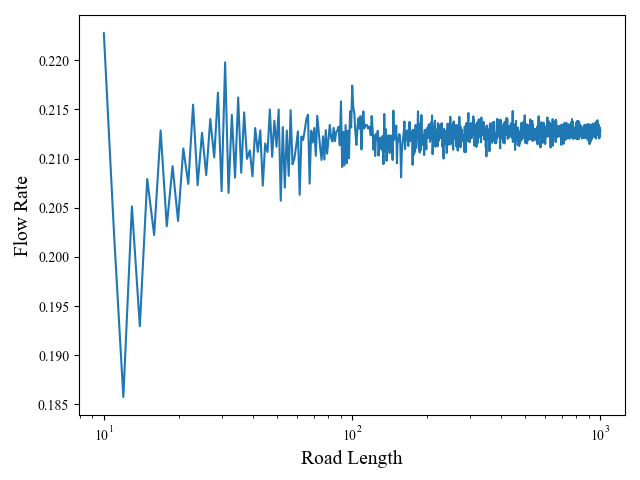
\includegraphics[width=1.\linewidth]{road.png}
        \begin{minipage}{0.8\textwidth}
            \captionof{figure}{Flow Rate vs Total Road Length}
            \label{fig:road_length}
        \end{minipage}
    \end{minipage}\hfill
    \begin{minipage}{.5\textwidth}
        \centering
        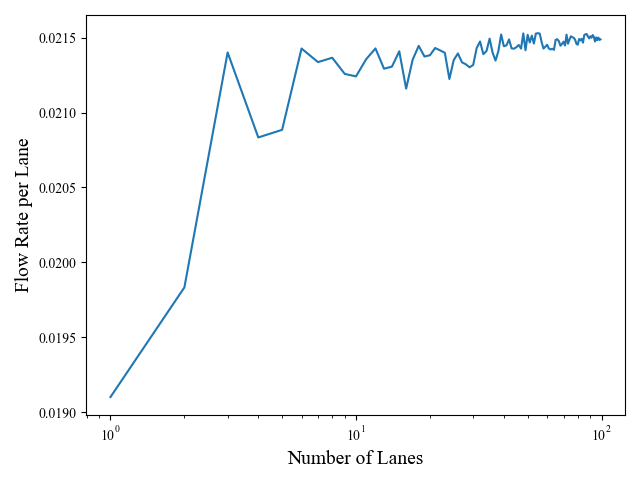
\includegraphics[width=1.\linewidth]{lanes.png}
        \begin{minipage}{0.8\textwidth}
            \captionof{figure}{Flow Rate per Lane vs Lane Count}
            \label{fig:lane_count}
        \end{minipage}
    \end{minipage}
\end{figure}

\begin{figure}[H]
    \centering
    \begin{minipage}{.5\textwidth}
        \centering
        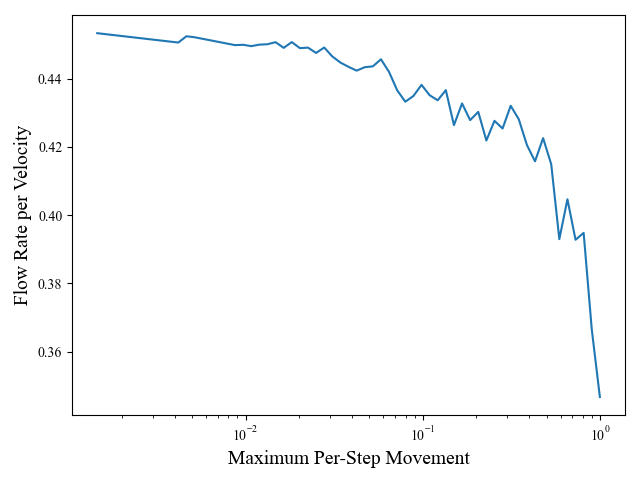
\includegraphics[width=.9\linewidth]{step_movement.png}
        \begin{minipage}{0.8\textwidth}
            \captionof{figure}{Flow Rate vs Maximum Per-Step Movement}
            \label{fig:step_movement}
        \end{minipage}
    \end{minipage}\hfill
    \begin{minipage}{.5\textwidth}
        \centering
        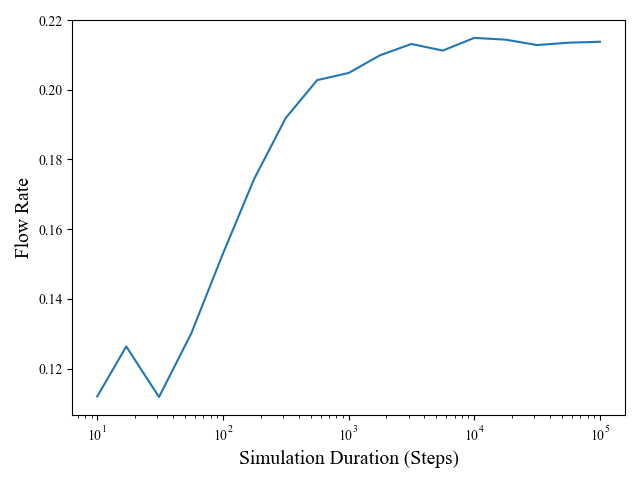
\includegraphics[width=1.\linewidth]{steps.png}
        \begin{minipage}{0.8\textwidth}
            \captionof{figure}{Flow Rate vs Simulation Duration}
            \label{fig:steps}
        \end{minipage}
    \end{minipage}
\end{figure}

\subsection{Lane Evaluation Strategy}

\begin{figure}[H]
    \centering
    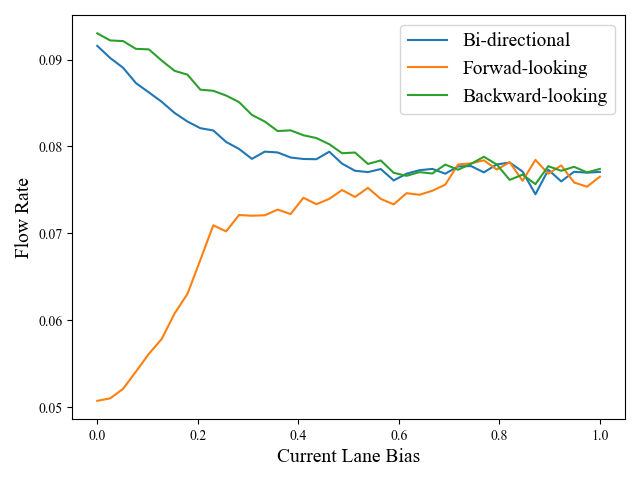
\includegraphics[width=0.8\textwidth]{methods-bias.png}
    \begin{minipage}{0.8\textwidth}
        \caption{Flow Rate vs Current Lane Bias for different Lane Evaluation Strategies}
        \label{fig:lane_strategy_bias}
    \end{minipage}
\end{figure}

\begin{figure}[H]
    \centering
    \begin{minipage}{.5\textwidth}
        \centering
        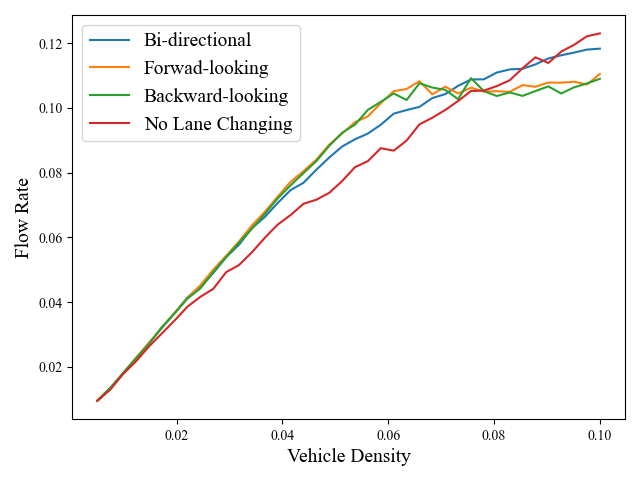
\includegraphics[width=1\textwidth]{methods-density.png}
        \begin{minipage}{0.8\textwidth}
            \caption{Flow Rate vs Vehicle Density for different Lane Evaluation Strategies}
            \label{fig:lane_strategy_density}
        \end{minipage}
    \end{minipage}\hfill
    \begin{minipage}{.5\textwidth}
        \centering
        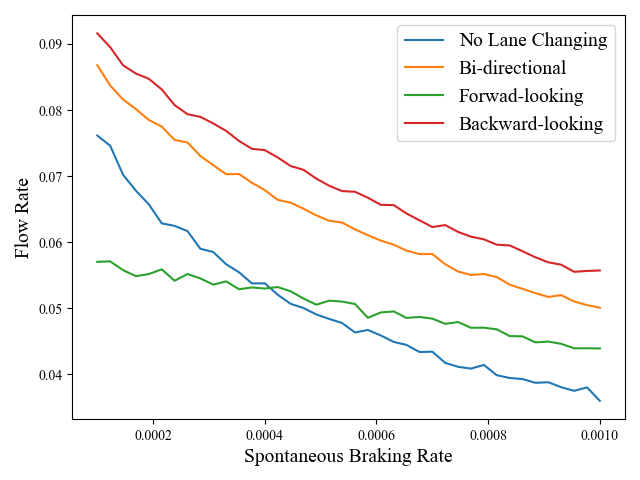
\includegraphics[width=1\textwidth]{methods-stop.png}
        \begin{minipage}{0.8\textwidth}
            \caption{Flow Rate vs Spontaneous Braking Rate for different Lane Evaluation Strategies}
            \label{fig:lane_strategy_stop}
        \end{minipage}
    \end{minipage}
\end{figure}

\begin{figure}[H]
    \centering
    \begin{minipage}{.5\textwidth}
        \centering
        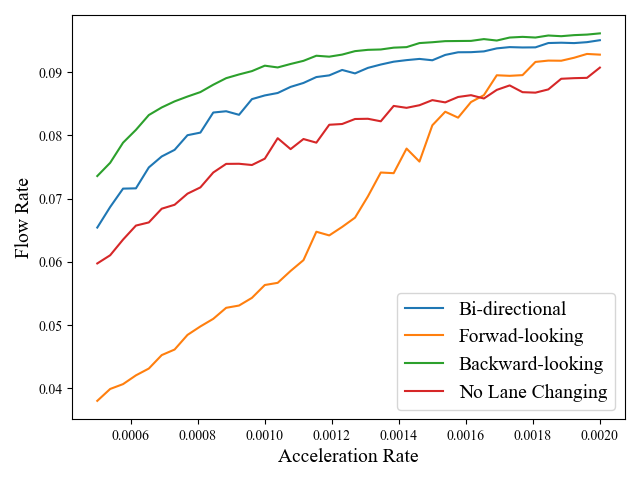
\includegraphics[width=1\textwidth]{methods-acceleration.png}
        \begin{minipage}{0.8\textwidth}
            \caption{Flow Rate vs Acceleration Rate for different Lane Evaluation Strategies}
            \label{fig:lane_strategy_acceleration}
        \end{minipage}
    \end{minipage}\hfill
    \begin{minipage}{.5\textwidth}
        \centering
        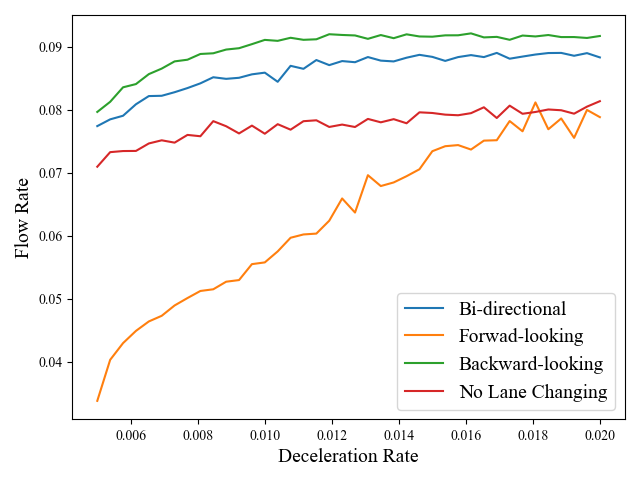
\includegraphics[width=1\textwidth]{methods-braking.png}
        \begin{minipage}{0.8\textwidth}
            \caption{Flow Rate vs Deceleration Rate for different Lane Evaluation Strategies}
            \label{fig:lane_strategy_braking}
        \end{minipage}
    \end{minipage}
\end{figure}

\section{Discussion}

The comparative analysis of different lane-changing strategies, as illustrated in Figures \ref{fig:lane_strategy_bias}, \ref{fig:lane_strategy_density}, \ref{fig:lane_strategy_stop}, \ref{fig:lane_strategy_acceleration}, and \ref{fig:lane_strategy_braking}, consistently ranks these strategies in terms of traffic flow rate as follows:

\begin{enumerate}
\item Backward-Looking
\item Bi-directional
\item No Lane Changing
\item Forward-Looking
\end{enumerate}

\subsection{Interpretation of ranking}
This ranking may be attributed to the distribution of vehicle velocities in the simulation. Predominantly, vehicles travel close to the maximum velocity, with only a minority at significantly lower speeds. This is due to infrequent occurrences of abrupt braking to a complete stop, leading to a scenario where most vehicles maintain high speeds.

The Forward-Looking strategy prompts vehicles approaching slower ones to change lanes. Given the prevalence of faster vehicles, this results in a higher number of lane changes. In contrast, the Backward-Looking strategy encourages slower vehicles to change lanes when faster vehicles approach, which, due to the lesser number of slow vehicles, results in fewer lane changes.

However, excessive lane changes can be problematic. Simultaneous lane changes by two vehicles, without considering each other, can lead to suboptimal or even hazardous situations, including potential collisions. This issue is particularly pronounced with the Forward-Looking strategy in environments where fast vehicles outnumber slow ones.

Interestingly, Figure \ref{fig:lane_strategy_acceleration} challenges this interpretation. Here, the Forward-Looking strategy outperforms the No Lane Changing strategy even with higher acceleration rates, which should theoretically lead to more fast vehicles and, consequently, a lower flow rate for the Forward-Looking strategy.

A plausible explanation for the superior performance of the Backward-Looking strategy lies in its consideration of vehicles behind it in the new lane, enhancing stability and reducing the likelihood of chain reactions in lane changes. The Forward-Looking strategy, lacking this consideration, may prompt a fast-approaching vehicle in the new lane to brake sharply and switch lanes, triggering a cascade of lane changes. Hence, the Backward-Looking strategy's inherent stability and its ability to mitigate chain reactions make it a more effective approach in maintaining traffic flow.

However, Figure \ref{fig:lane_strategy_stop} presents a counterpoint to this interpretation. In scenarios of higher Spontaneous Braking Rates, the Forward-Looking strategy not only outperforms the No Lane Changing strategy but also exhibits the least reduction in flow rate as the braking rates increase. Contrary to the expectation that more frequent braking would lead to a greater number of lane-change cascades under the Forward-Looking strategy, the data from \ref{fig:lane_strategy_stop} suggests otherwise. It is important to note, though, that the Backward-Looking strategy still maintains superior performance compared to the Forward-Looking strategy under conditions of high Spontaneous Braking Rates.

The most coherent interpretation of the data suggests that the Forward-Looking strategy is inherently less stable compared to the others, leading to its overall inferior performance. Nonetheless, it does show marginally improved effectiveness in scenarios where there is a greater variance in vehicle velocities.

The Forward-Looking strategy engages in lane changes primarily when encountering vehicles moving slower ahead, without accounting for the impact on vehicles behind. This approach, while individually effective, can be seen as less collaborative when compared to the Backward-Looking strategy. The Backward-Looking strategy, in contrast, is more considerate of the following vehicles, initiating lane changes when it is moving slower than the surrounding traffic. This more cooperative behavior tends to promote a more stable traffic pattern and leads to an increased overall flow rate.

\subsection{Optimal Current Lane Bias}
Figure \ref{fig:lane_strategy_bias} reveals that the default setting for Current Lane Bias was not optimal for maximizing traffic flow. Interestingly, the optimal value for Current Lane Bias seems to be at the extremes, either 0 or 1, varying with the lane-changing strategy employed. This finding implies that Current Lane Bias has a minimal impact on flow rate, and it is the lane-changing strategy itself that plays a more significant role.

This could be because in our model, lane changes are immediate, lacking a transition period, which makes changing lanes effortless. In this context, a car can change lanes just as easily as staying in its current lane. Switching to a less optimal lane is just as disadvantageous as remaining in one. With no cost associated with changing lanes, setting the bias to 0 is most effective when lane changing offers an advantage.

The primary drawback of frequent lane changes is the potential for chaos in high-density traffic environments. This is because multiple vehicles might attempt to change lanes simultaneously, which could hinder the effectiveness of the lane-changing strategy. In such scenarios, excessive lane changes could lead to reduced efficiency and potential traffic disruptions. This phenomenon is evident in Figure \ref{fig:lane_strategy_density}, where the flow rates for all lane-changing strategies tend to converge to a similar value at higher vehicle densities. This convergence suggests that the benefits of different lane-changing strategies diminish as traffic density increases.

\subsection{Effect of Vehicle Density}
Figure \ref{fig:lane_strategy_density} indicates that the distinctions among different lane-changing strategies become less marked at very low and very high vehicle densities. This observation aligns with intuition: at low densities, there is less need for vehicles to change lanes frequently, while at high densities, the limited available space restricts the ability of vehicles to maneuver between lanes.

\newpage
\section{Conclusion}
Lane changing proves advantageous only when the surrounding conditions, particularly vehicle density. Under ideal conditions, the optimal approach involves being considerate of other vehicles, as shown by the superios Backward-Looking strategy. In this model, the optimal approach includes changing lanes as necessary, given that there is no penalty associated with lane changes. However, it's crucial that the vehicle density is appropriate for this strategy to be effective. This contrasts with real-world driving, where lane changes require time and can impact traffic flow in complex ways.

\end{document}
